\documentclass[twocolumn, a4paper]{icethesisabst}
\usepackage[dvipdfmx]{graphicx}
%\renewcommand{\figurename}{Fig.}

\title{{\bf 卒業研究概要書の題目}
  {\normalsize \\ Title of the thesis}}
  \author{
    AF16009 池辺~颯一 \\ Soichi Ikebe \and
    指導教員 神澤~雄智 \\ Yuchi Kanzawa
  }

\begin{document}
\maketitle
\section{はじめに}
% ここでは,研究を着手するに至った背景~\cite{Kawasaki},
% 研究の目的~\cite{Yamada}に関して,具体的に述べる~\cite{Seki}.
% 特に,研究課題~(あるべき理想像)と現実とのギャップから問題点が何であるか
% を明確化し,その問題点を解決するためにどのような方法で,
% どこまで達成するのかをまとめる.
% 以下,本稿の書き方について触れる.原稿はA4サイズで作成する.
% マージンは上マージン30mm,左マージン19mm,右マージン22mm,下マージン27mmとする.
% フォントは,原則としてタイトルと各節の見出しはゴシック系フォントとし,
% 著者名と本文は明朝系フォントを用いること.
% フォントサイズは,タイトルは16ポイント,その他は9ポイントとする.
% Fig.~\ref{fig:sample}に参考図を示す.
% 他のワードプロセッサ等で作成する場合は,これらの数値を参考にすること.
% \begin{figure}[htbp]
%  \centering
% \includegraphics[width=\linewidth]{fig.eps}
% \caption{Current and Temperature as Functions of Applied Voltage.}
% \label{fig:sample}
% \end{figure}

% \begin{enumerate}
%  \item
% 複数人の共同研究であっても1人ずつ~(1枚ずつ)提出すること.
% また,自分が中心に行ったことをまとめるので,全く同じ原稿は認めない.
% \item
% 研究題目は抽象的な表現を用いず,実際の研究内容を具体的に表したものにする
%      こと.
% 英文併記.
% \item
% 指導教員名は「姓名」のみを記入すること.著者名(学生名と指導教員名)は英文併記.
% \item
% 形式は,「はじめに」「研究内容」「研究成果」「まとめと今後の課題」「参考
%      文献」
% などの順で書く.謝辞はまとめの中で書くこと.
% ただし,各節のタイトルは研究内容に応じて適切に変更してよい.
% \item
% 図の番号およびキャプションは図の下に書き,
% 表の番号およびキャプションは表の上に書くこと.
% \item
% 図表内文言は可能な限り英語表記とすること.また,図表のタイトルは日本語表記の下に
% 英文表記を併記すること.
% \item
% 文中で図表を説明する際には「図1に○○を示す」のように日本語の図表番号を用いること.
% \item
% 仕上がりは,グレースケールではなく白黒であることに注意して図を作成するこ
%      と.
% \item
% 使用フォントを全て埋め込んだPDFファイルとして提出すること.
% \item
% ファイルサイズは5Mバイト以下とすること.
% \item
% 共同研究者がいる場合は,自分の名前の後ろに学籍番号とともに記述すること.
% \item
% 不明な点は指導教員に確認すること.
% \end{enumerate}


近年,情報通信社会の発展に伴いデータ量が増大し,
日々多様なデータがコンピュータに蓄積されている.
この大量のデータから有益な情報を抽出する手法として,
データを類似度に基づきグループ化するクラスタリングに注目が集まっている.
既存の手法における課題として,各クラスタのサイズに差がある場合,
クラスタリングから有意な結果が得られないというものがある.
そこで,各クラスタのサイズを考慮してクラスタリングを行う手法が複数提案されており,
本研究はそれらの手法について各手法の特性を把握するとともに,
最も有用な手法を発見することを目的とする.


\section{提案内容}
% 提案技術の具体的内容に関して,
% 図表などを用いて分かりやすく述べる.
% また,図を挿入する場合は,カラーは用いず白黒で描くこと.
% カラーやグレースケールを用いた図や写真は,
% 印刷時に諧調がつぶれて真っ黒になってしまう可能性があるので特に注意すること.

各クラスタのサイズを考慮するために,
既存の手法にクラスタサイズ調整変数を導入した以下の3手法について実験を行う.
\begin{itemize}
 \item eFCMA
 \item qFCMA
 \item sFCMA
\end{itemize}

まず,これらの手法についてそれぞれの特性を把握するため,人工データを用いて実験を行う.
複数のパラメータで実験を行い,それぞれで算出された分類関数から比較及び評価を行う.

次に,これらの手法から最も有用なものを発見するために,
実データを用いてARI(Adjusted Rand Index)を算出し,
その値が最も高いものを有用な手法と評価する.

\section{研究成果}
% 問題点の解決に関して,
% 提案技術が既存技術と比較してどの程度有効であるか定量的に述べる.

人工データとして,
クラス数2,各クラスのデータ数50,合計データ数100のデータを
平均値($-1$, $-1$),標準偏差($0.5$, $0.5$)
及び平均値($1$, $1$),標準偏差($0.5$, $0.5$)
のガウスサンプリングで生成したデータを用いた(図~\ref{fig:a_data}).

\begin{figure}[htbp]
\centering
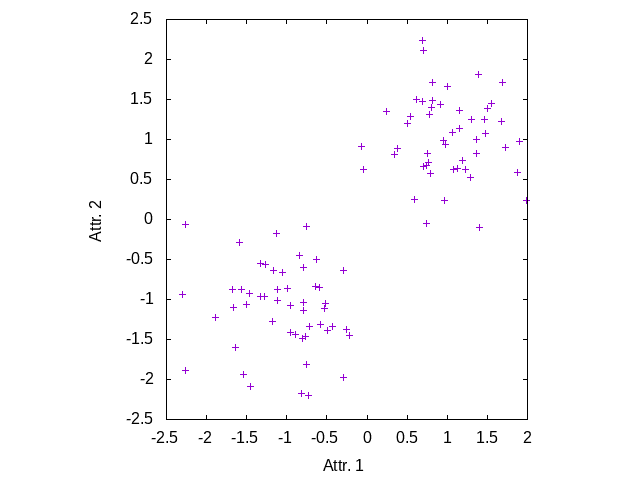
\includegraphics[width=6.5cm]{2d-dat.png}
\caption{人工データ}
\label{fig:a_data}
\end{figure}

\section{まとめと今後の課題}
% 本研究の成果を簡潔にまとめるとともに,どのような
% 課題が今後検討されなければならないかについて述べる.

\begin{thebibliography}{99}
\bibitem{Kawasaki}
河崎めぐみ,千葉翔太:
``加速度センサーを用いたユーザの行動状態推定方式,''
信学論B, Vol.~J85-B, No.~5, pp.~755--767, (2011).
\bibitem{Yamada}
山田一郎,中村仁:
``モバイル環境におけるマルチメディア通信品質の研究,''
信学技報, Vol.~109, No.~204, pp.~27--32, (2010).
\bibitem{Seki}
Seki, Y. and Kirii, Y.:
``Fast Handover Scheme using User's preference, ''
Wireless Communications and Mobile Computing,
Vol.~7, Issue~5, pp.~553--568, (2009).
\end{thebibliography}
\end{document}
